Тестирование реализованного алгоритма на блочно-структурированных сетках проводилось на задаче \eqref{eq:problem_3}.
Так как проводилось исследование работоспособности именно блочности сетки, а не её динамической адаптации, был выбран отрезок времени $t \in [40, 42]$.
На \figref{fig:block_structured_grid} представлена сетка, на которой проивоздился расчёт.
\begin{figure}[h]
    \centering
    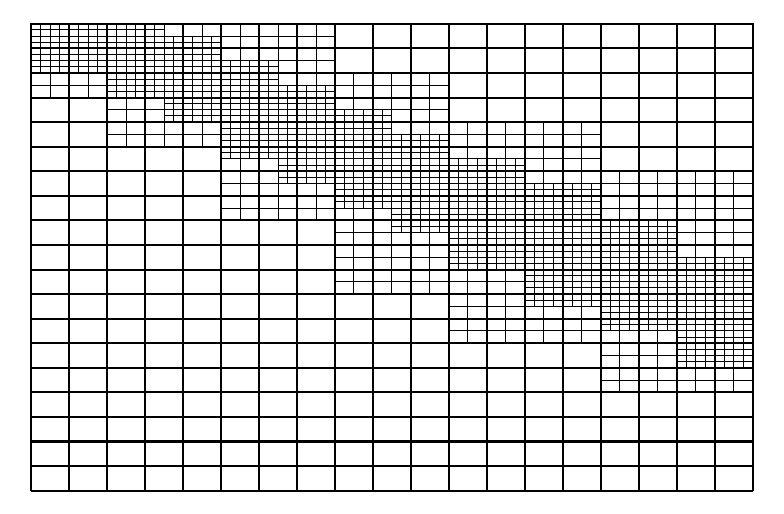
\includegraphics[width=\textwidth, height=\textheight, keepaspectratio]{Теория_блочных_локально_адаптивных_сеток/Результаты_моделирования/grid.pdf}
    \caption{Блочно-структурированная сетка, учитывающая особенность решения}
    \label{fig:block_structured_grid}
\end{figure}
Из рисунка видно, что самая грубая сетка соответствует выбору числа точек $N_x = 41$ и $N_y = 21$.
График ошибок численного решения, полученного только на грубой сетке, приведён на \figref{fig:coarse_errors}
\begin{figure}
    \centering
    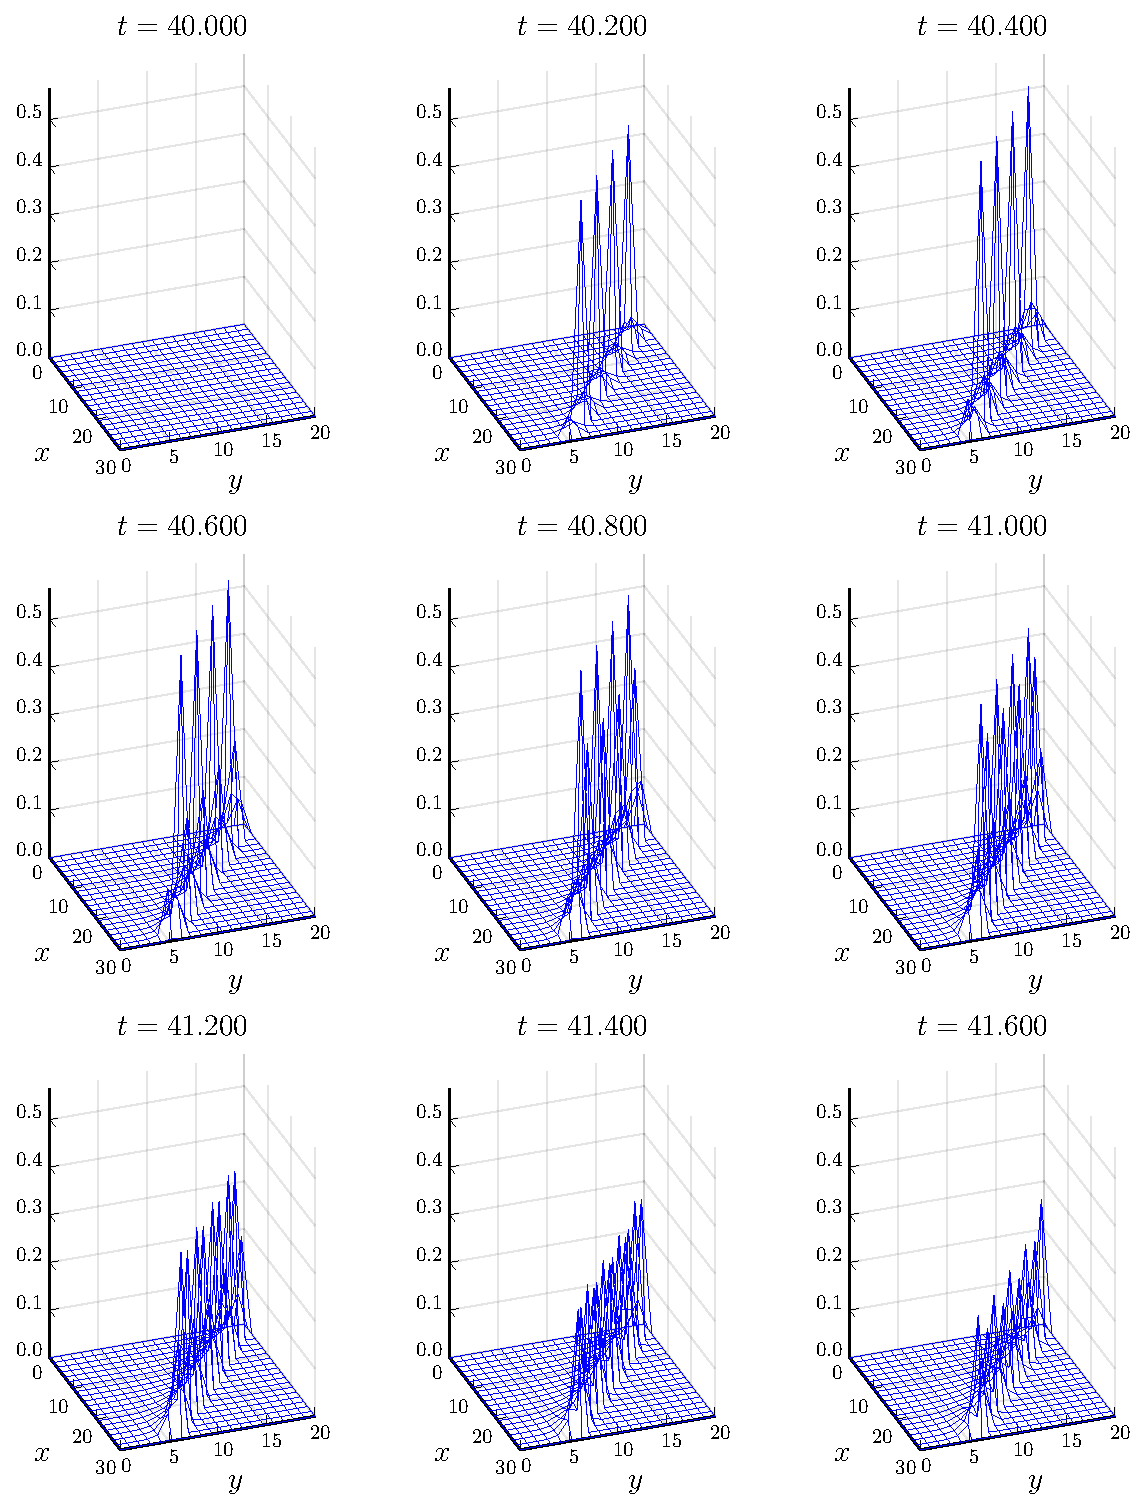
\includegraphics[width=\textwidth, height=\textheight, keepaspectratio]{Теория_блочных_локально_адаптивных_сеток/Результаты_моделирования/errors_before.pdf}
    \caption{График ошибок численного решения на грубой сетке $N_x = 41, N_y = 21$.}
    \label{fig:coarse_errors}
\end{figure}
График ошибок численного решения, полученного при использовании описанного выше алгоритма на стрктурированной сетке приведён на \figref{fig:structured_errors}
\begin{figure}
    \centering
    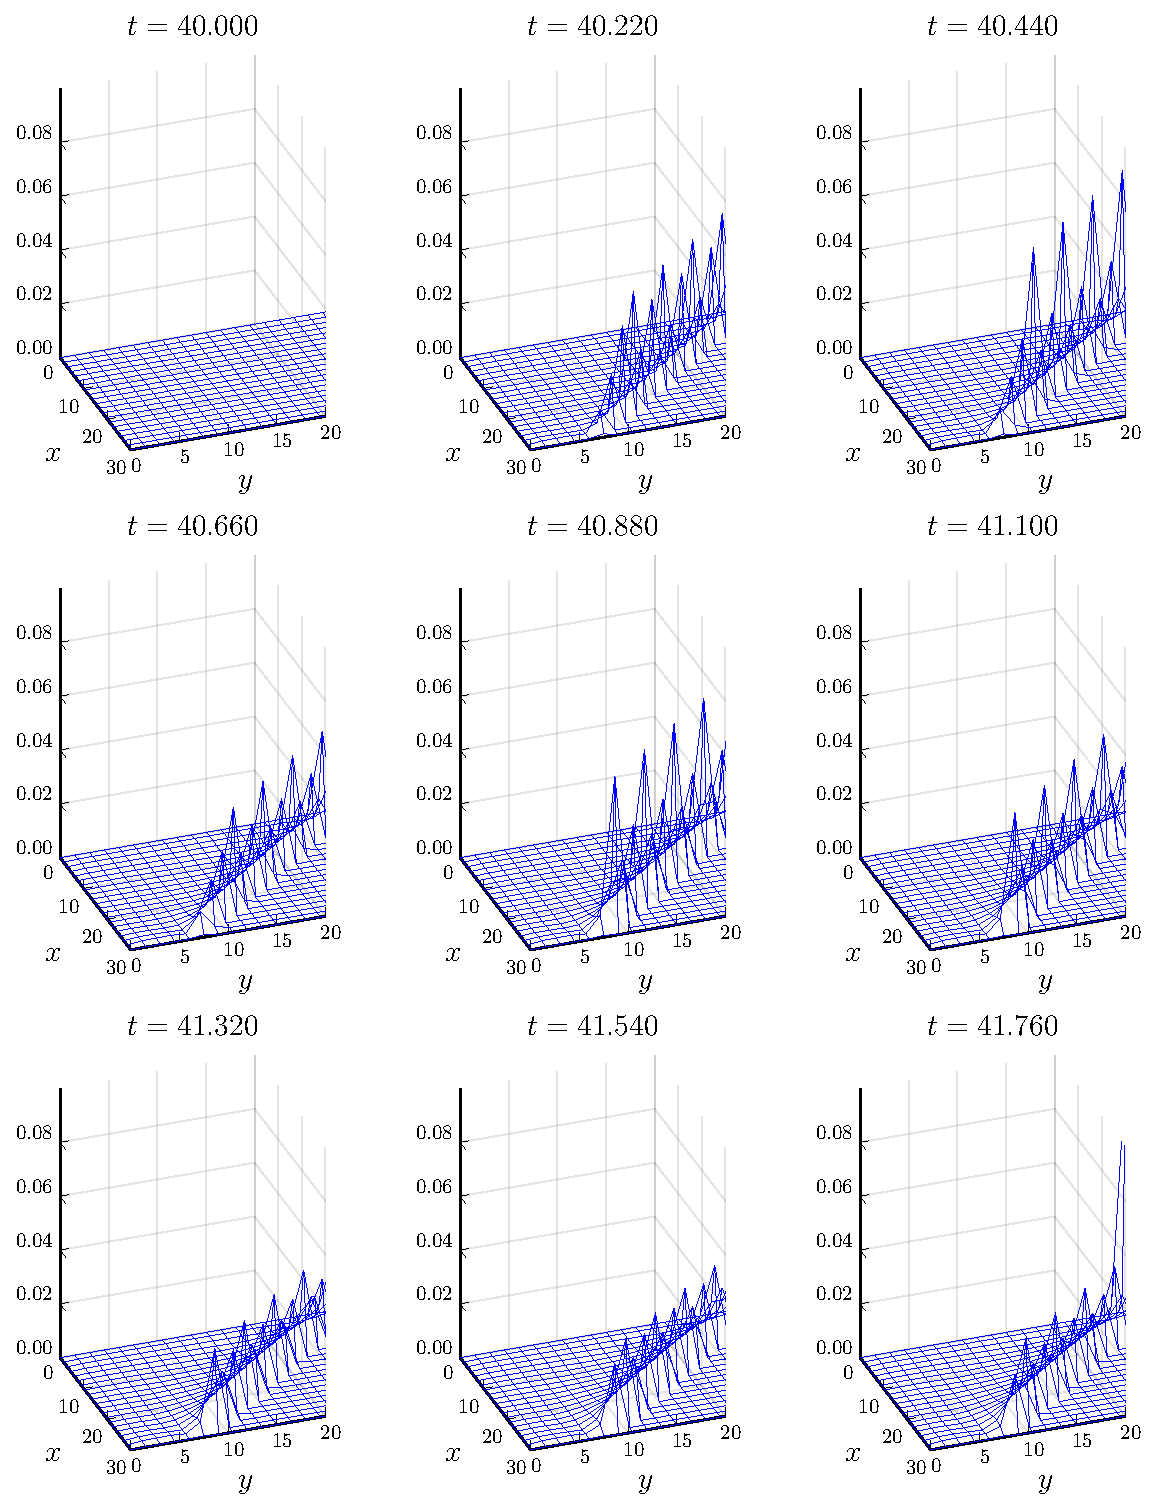
\includegraphics[width=\textwidth, height=\textheight, keepaspectratio]{Теория_блочных_локально_адаптивных_сеток/Результаты_моделирования/errors_after.pdf}
    \caption{График ошибок численного решения на блочно-структурированной сетке с тремя уровнями измельчения}
    \label{fig:structured_errors}
\end{figure}
Из него непосредственно видно, что ошибка вблизи особенностей заметно уменьшилась.
Также видно большее \glqq размытие\grqq окрестности особенности решения.
Это указывает на то, что такая сетка \glqq размывает\grqq пики вблизи разрывов, делая погрешность решения более равномерной по всей области (что и соответствует тому, что мы находим решение с заданной точностью во всей области сразу).
Также сравнивалось время, затраченное на расчёт на такой блочно-структурированной сетке и на равномерной сетке, соответствующей самому мелкому разбиению из блочно-структурированной сетки: производительность первой программы оказалась $\approx$ в 10 раз выше.
Таким образом, показаны основные достоинства реализованного алгоритма.

\begin{wrapfigure}{r}{0.3\textwidth}
    \begin{center}
        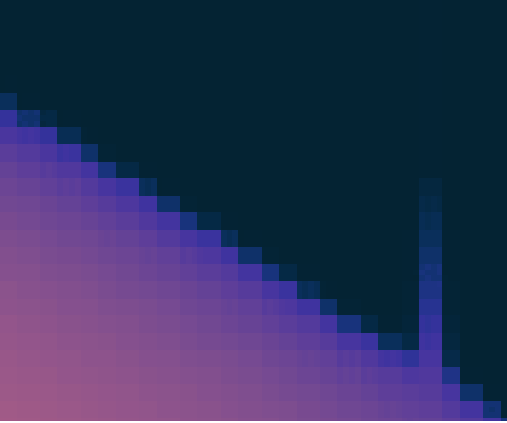
\includegraphics[width=0.25\textwidth, height=0.4\textheight, keepaspectratio]{Теория_блочных_локально_адаптивных_сеток/Результаты_моделирования/artifact.png}
    \end{center}
    \caption{Недочёты алгоритма}
    \label{fig:artifacts}
\end{wrapfigure}
В процессе разработки и тестирования были найдены ошибки и недочёты программы, а именно, при достаточно большом количестве блоков и при их небольшом размере возможно возникновение так называемых артефактов решения (\seefigref{fig:artifacts}), появляющихся на стыках двух блоков одного уровня.
Скорее всего, данная особенность возникает из-за не совсем корректного учёта синхронизации данных на двух блоках.
Точная причина и пути её устранения ещё подлежат дальнейшему анализу.